\chapter{Classification results evaluation} \label{chapt4}
\section{Base line model} \label{sect4_2}
It is a common knowledge that RNN based neural networks shows the best performance for the text based problems. For my goal, I used Bidirectional Long-Short Term Memory (bi-LSTM) model with 100 ... HERE DESCRIBE MORE ABOUT PARAMETERS 


\begin{figure}[ht] 
	\center
	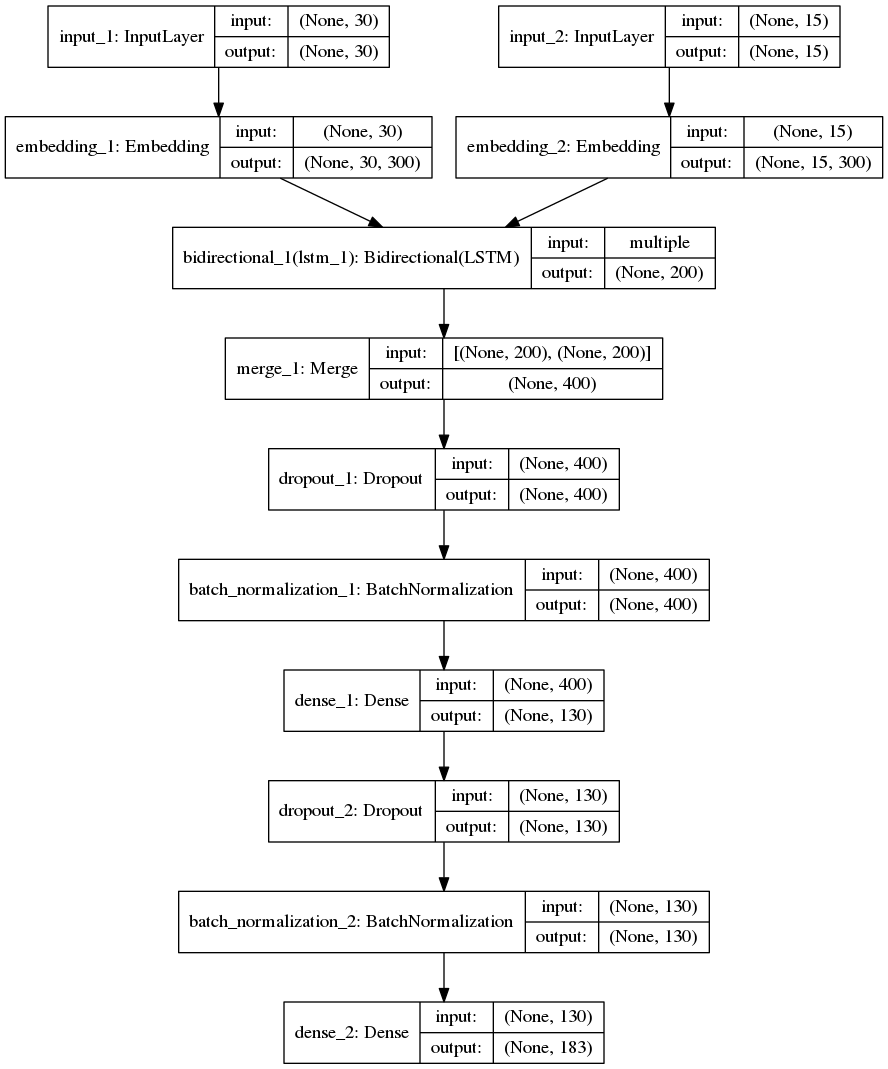
\includegraphics [scale=0.4] {part4/bilstm_architecture.png}
	\label{img:part4-bilstm}  
	\caption{Architectures of Bi-LSTM models with 100 units } 
\end{figure}



top\_k\_categorical\_accuracy


\begin{figure}[ht]
	\begin{minipage}[ht]{1\linewidth}
		\center{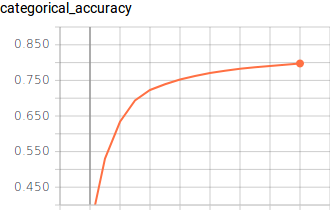
\includegraphics[width=0.5\linewidth]{part4/bilstm_train_category_accuracy}}
	\end{minipage}
	\hfill
	\begin{minipage}[ht]{1\linewidth}
		\center{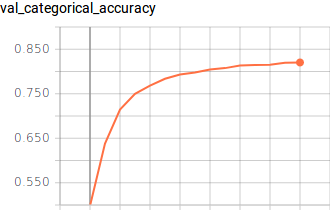
\includegraphics[width=0.5\linewidth]{part4/bilstm_val_category_accuracy}}
	\end{minipage}
	\caption{Models train and validation categorical accuracy by epochs}
	\label{img:categorical_accuracy}  
\end{figure}

\begin{figure}[ht]
	\begin{minipage}[ht]{1\linewidth}
		\center{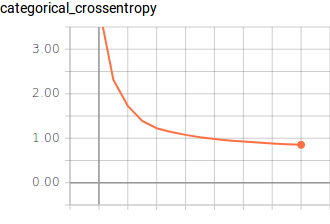
\includegraphics[width=0.5\linewidth]{part4/bilstm_train_category_crossentropy}}
	\end{minipage}
	\hfill
	\begin{minipage}[ht]{1\linewidth}
		\center{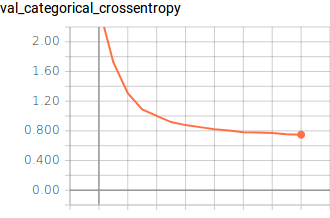
\includegraphics[width=0.5\linewidth]{part4/bilstm_val_category_crossentropy}}
	\end{minipage}
	\caption{Models train and validation category crossentropy by epochs}
	\label{img:category_crossentropy}  
\end{figure}

\begin{figure}[ht]
	\begin{minipage}[ht]{1\linewidth}
		\center{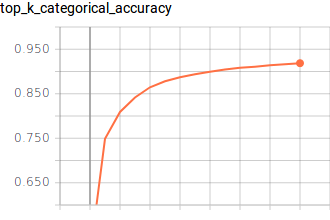
\includegraphics[width=0.5\linewidth]{part4/bilstm_train_top_k_accuracy}}
	\end{minipage}
	\hfill
	\begin{minipage}[ht]{1\linewidth}
		\center{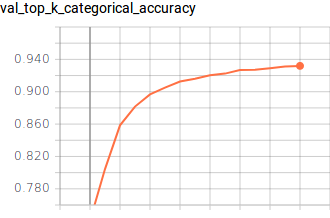
\includegraphics[width=0.5\linewidth]{part4/bilstm_val_top_k_accuracy}}
	\end{minipage}
	\caption{Models train and validation top k accuracy by epochs}
	\label{img:category_crossentropy}  
\end{figure}

\begin{figure}[ht] 
	\center
	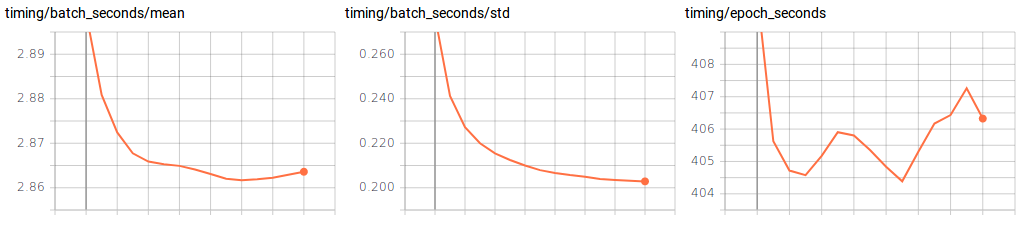
\includegraphics [scale=0.5] {part4/bilstm_timing}
	\caption{Models batch time by epochs} 
	\label{img:bilstm_timing}  
\end{figure}


\begin{figure}[ht]
	\begin{minipage}[ht]{1\linewidth}
		\center{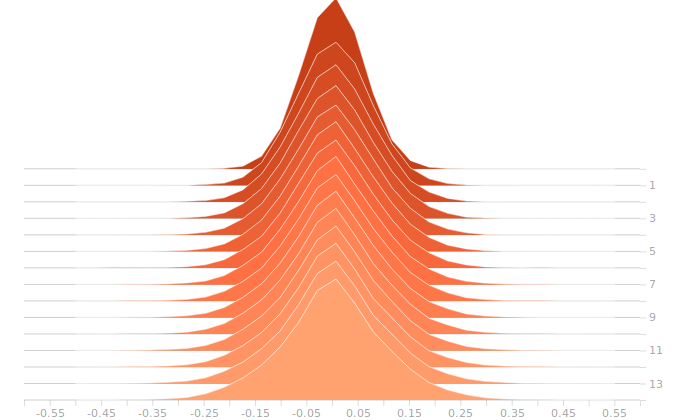
\includegraphics[width=0.5\linewidth]{part4/bilstm_forward_lstm_1_recurrent_kernel_0} \\ а}
	\end{minipage}
	\hfill
	\begin{minipage}[ht]{1\linewidth}
		\center{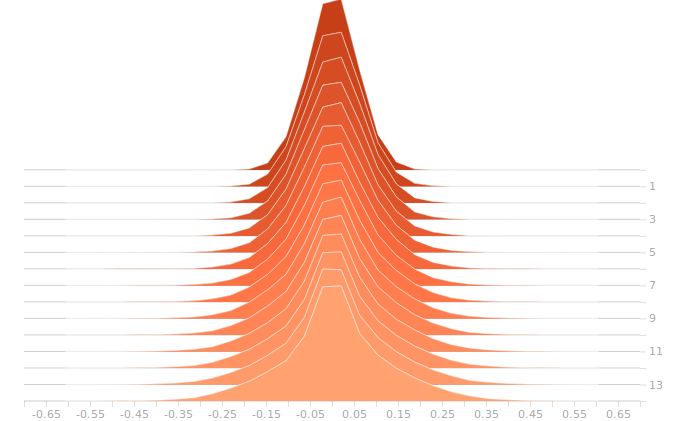
\includegraphics[width=0.5\linewidth]{part4/bilstm_backward_lstm_1_recurrent_kernel_0} \\ b}
	\end{minipage}
	\caption{Bi-LSTM 100 units. Histogram of output from forward recurrent layers (a); histogram of weights from backward recurrent layers (b)}
	\label{img:category_crossentropy}  
\end{figure}


\begin{figure}[ht] 
	\center
	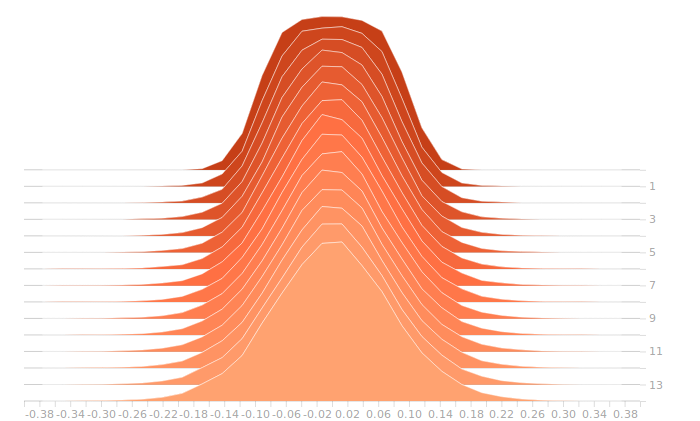
\includegraphics [scale=0.5] {part4/bilstm_dense}
	\caption{Bi-LSTM 100 units. Histogram of weights from first FFNN layer.} 
	\label{img:bilstm_dense}  
\end{figure}

\begin{figure}[ht] 
	\center
	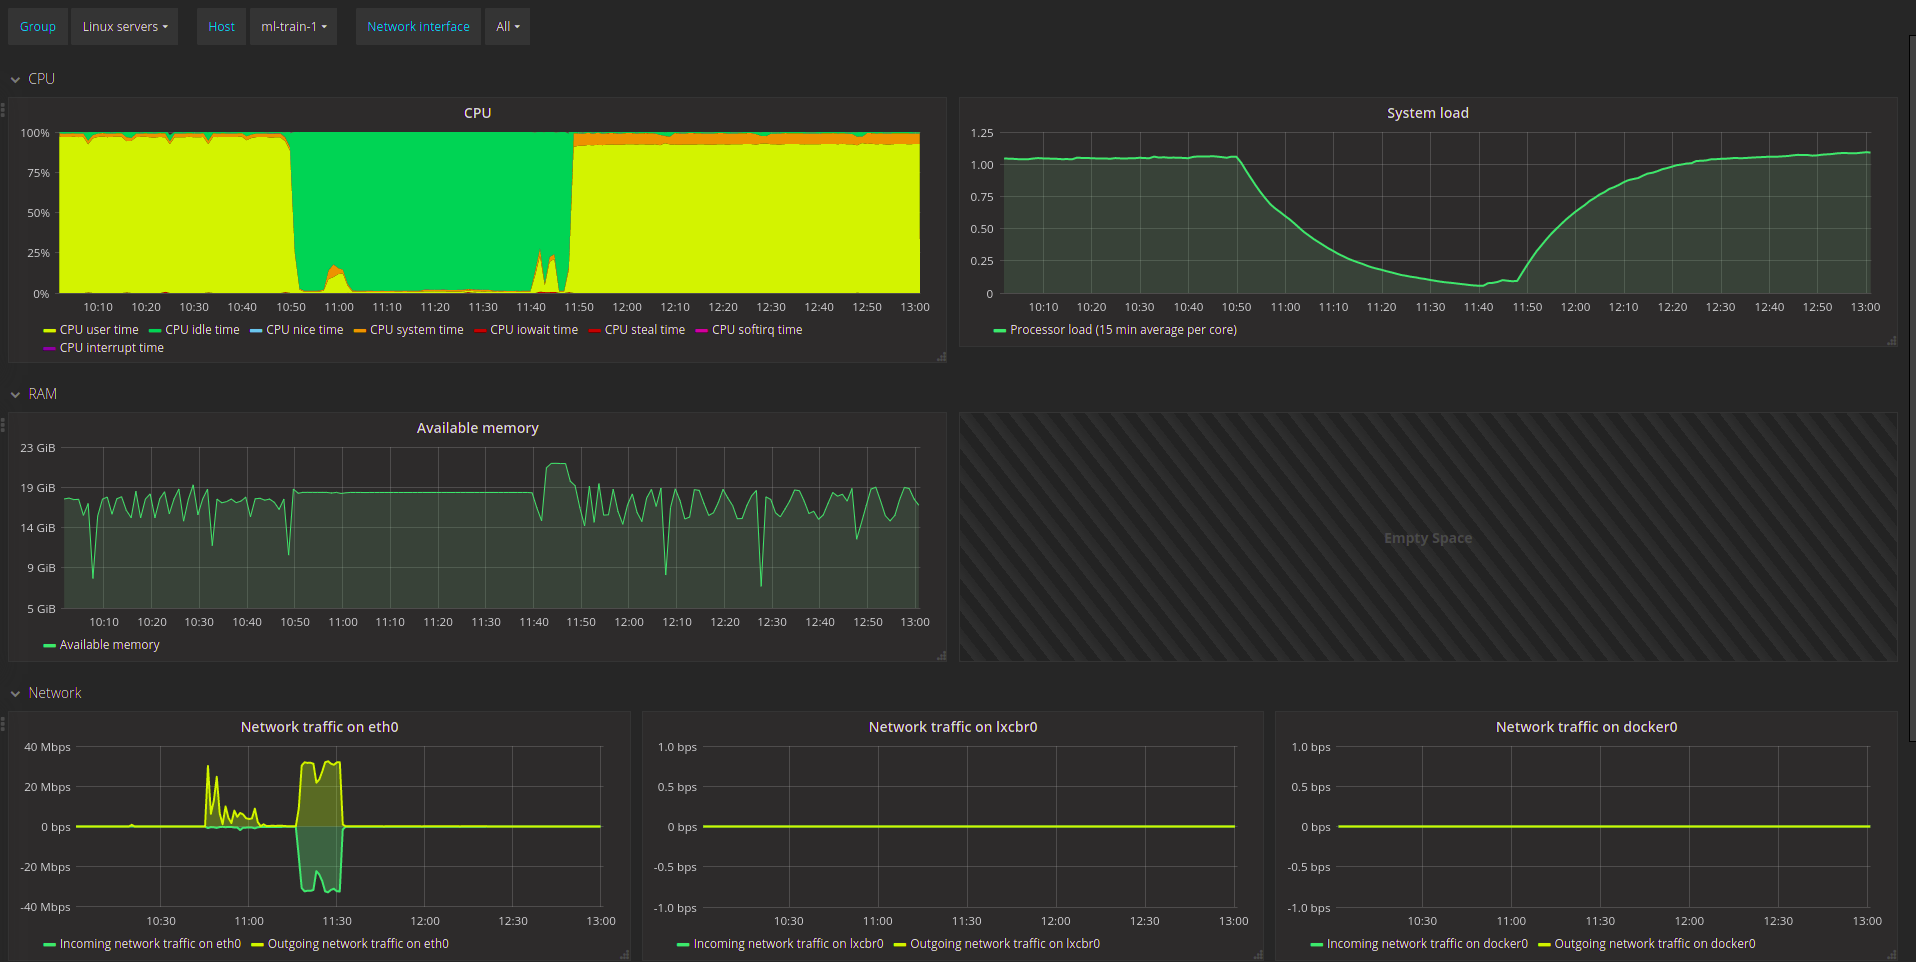
\includegraphics [scale=0.2] {part4/resources_BILSTM}
	\caption{CPU resources which were used while training Bi-LSTM NN.} 
	\label{img:resources_BILSTM}  
\end{figure}





\section{Convolution neural network} \label{sect4_2}

\begin{figure}[ht] 
	\center
	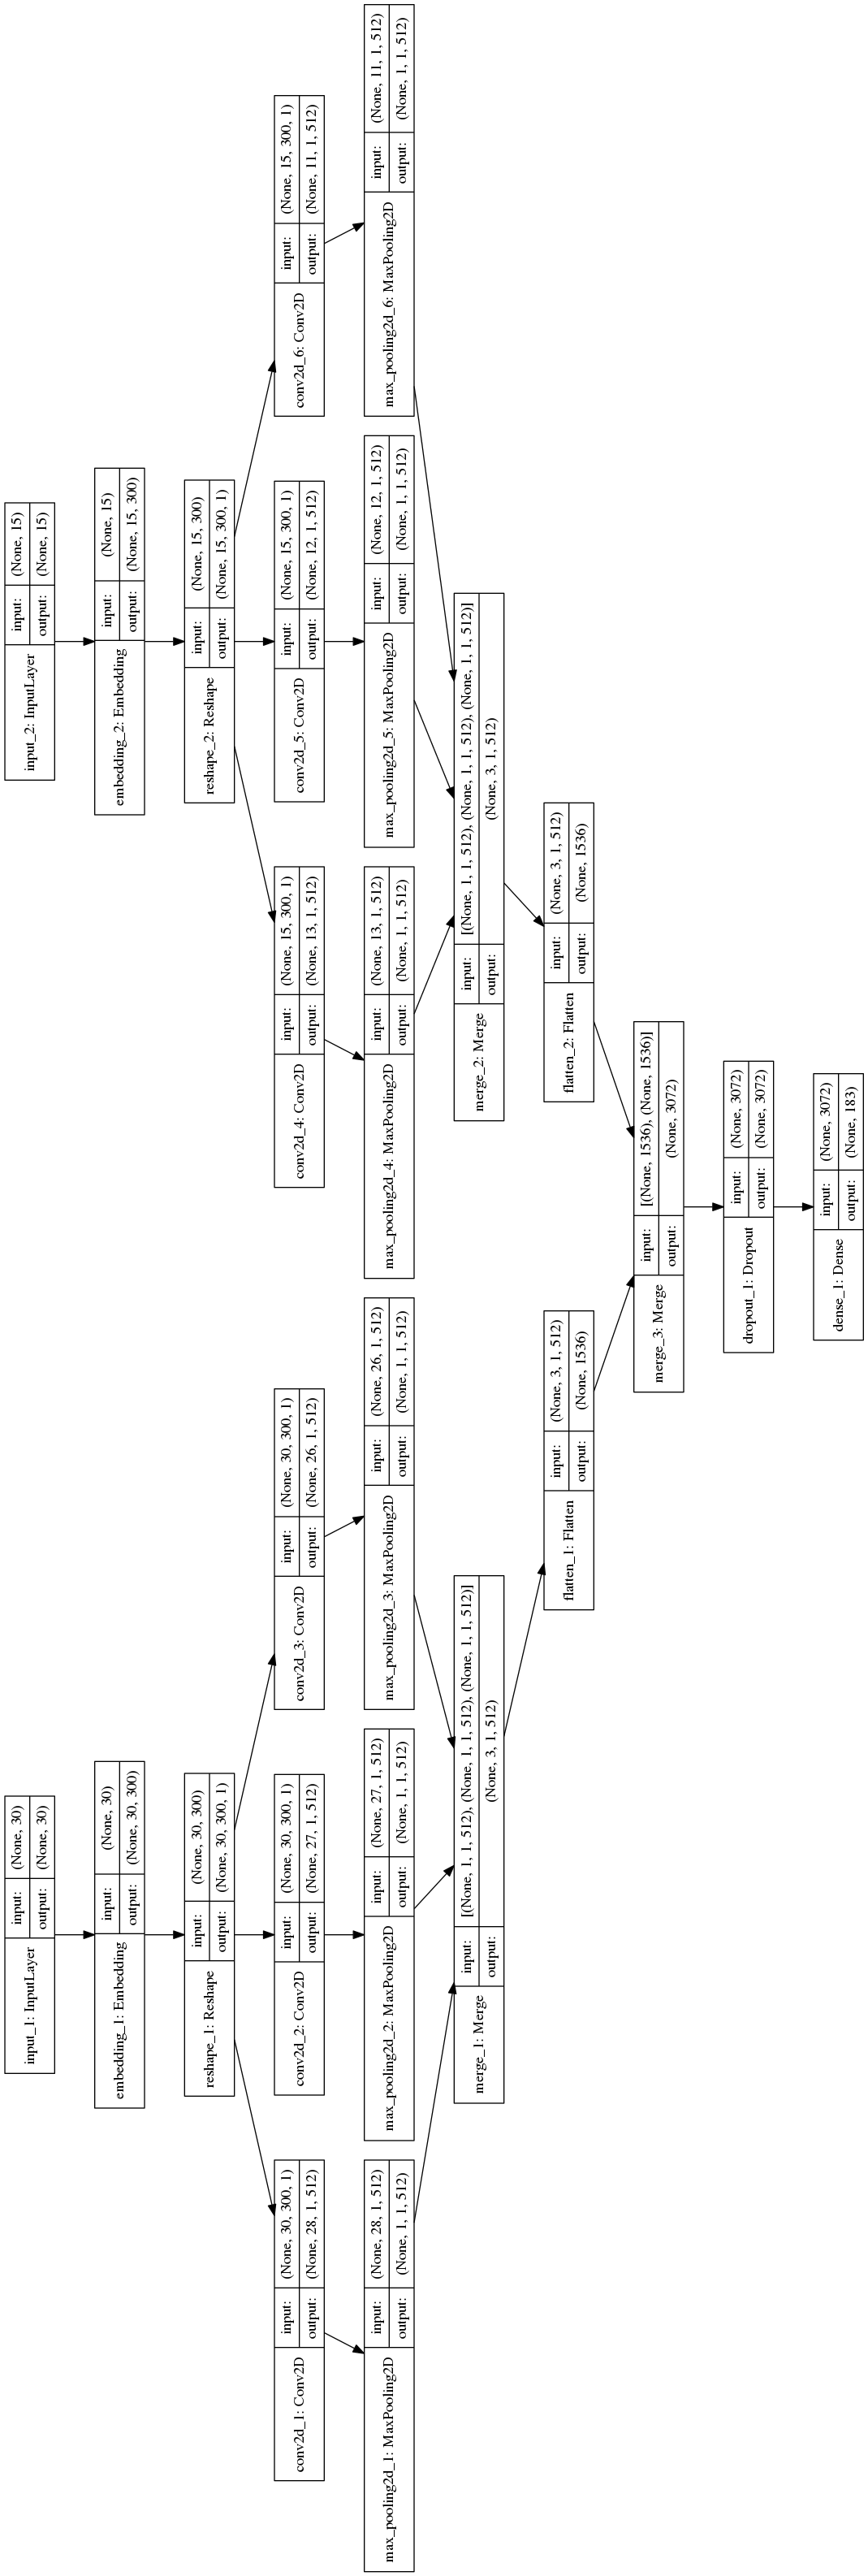
\includegraphics [scale=0.2] {part4/cnn_architecture.png}
	\label{img:cnn_architecture}  
	\caption{Architectures of CNN model} 
\end{figure}



top\_k\_categorical\_accuracy


\begin{figure}[ht]
	\begin{minipage}[ht]{1\linewidth}
		\center{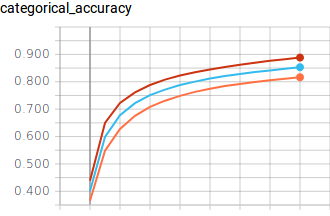
\includegraphics[width=0.5\linewidth]{part4/3CNN_train_category_accuracy}}
	\end{minipage}
	\hfill
	\begin{minipage}[ht]{1\linewidth}
		\center{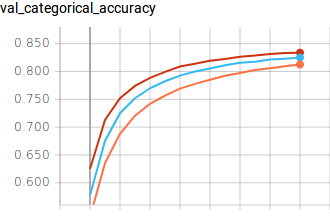
\includegraphics[width=0.5\linewidth]{part4/3CNN_val_category_accuracy}}
	\end{minipage}
	\caption{Models train and validation categorical accuracy by epochs}
	\label{img:3CNN_categorical_accuracy}  
\end{figure}


\begin{figure}[ht]
	\begin{minipage}[ht]{1\linewidth}
		\center{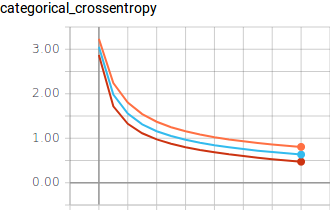
\includegraphics[width=0.5\linewidth]{part4/3CNN_train_category_crossentropy}}
	\end{minipage}
	\hfill
	\begin{minipage}[ht]{1\linewidth}
		\center{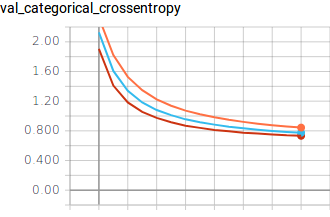
\includegraphics[width=0.5\linewidth]{part4/3CNN_val_category_crossentropy}}
	\end{minipage}
	\caption{Models train and validation category crossentropy by epochs}
	\label{img:3CNN_category_crossentropy}  
\end{figure}

\begin{figure}[ht]
	\begin{minipage}[ht]{1\linewidth}
		\center{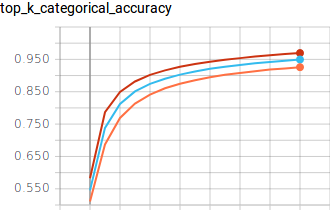
\includegraphics[width=0.5\linewidth]{part4/3CNN_train_top_k_accuracy}}
	\end{minipage}
	\hfill
	\begin{minipage}[ht]{1\linewidth}
		\center{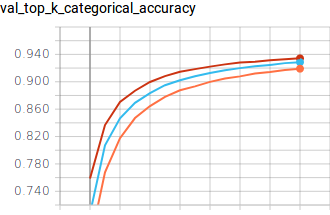
\includegraphics[width=0.5\linewidth]{part4/3CNN_val_top_k_accuracy}}
	\end{minipage}
	\caption{Models train and validation top k accuracy by epochs}
	\label{img:3CNN_top_k_accuracy}  
\end{figure}

\begin{figure}[ht] 
	\center
	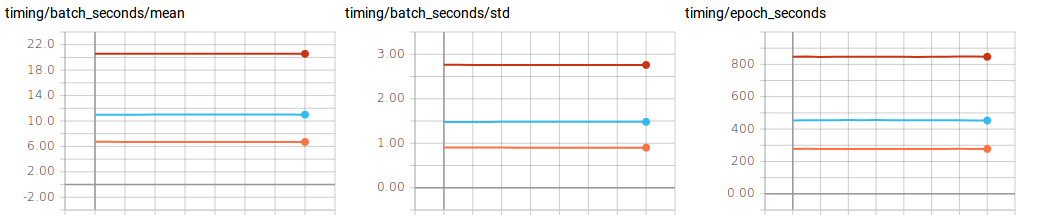
\includegraphics [scale=0.5] {part4/3CNN_timing}
	\caption{Models batch time by epochs} 
	\label{img:3CNN_timing}  
\end{figure}



\begin{figure}[ht]
	\begin{minipage}[ht]{1\linewidth}
		\center{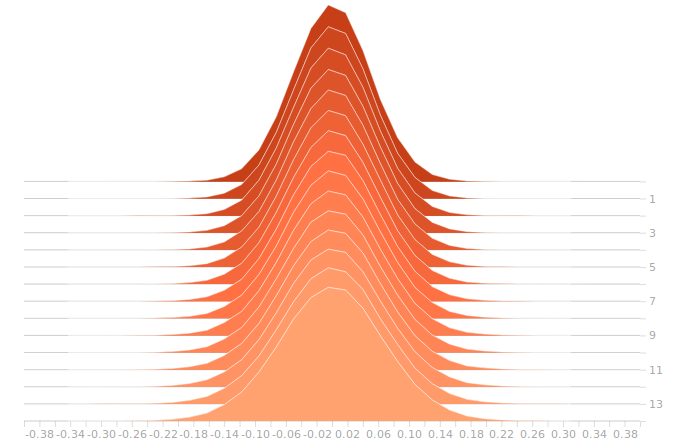
\includegraphics[width=0.5\linewidth]{part4/3CNN-conv-128.png} \\ а}
	\end{minipage}
	\hfill
	\begin{minipage}[ht]{1\linewidth}
		\center{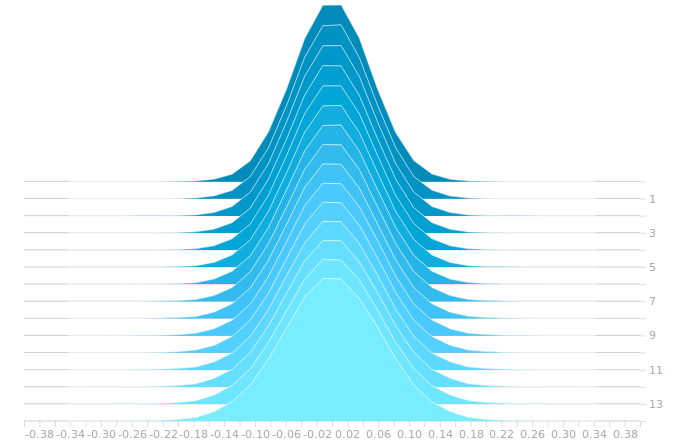
\includegraphics[width=0.5\linewidth]{part4/3CNN-conv-256.png} \\ b}
	\end{minipage}
	\begin{minipage}[ht]{1\linewidth}
		\center{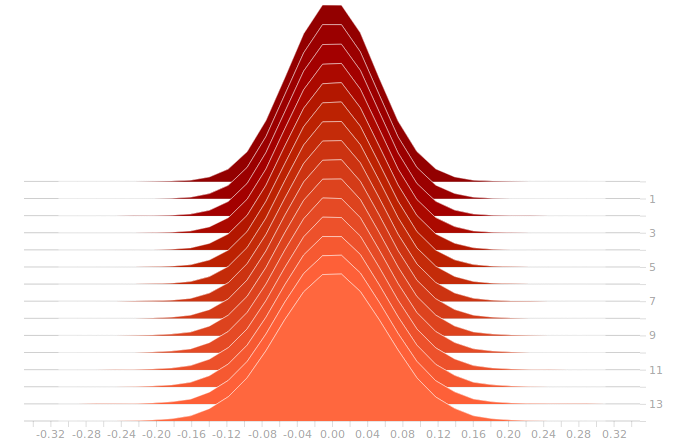
\includegraphics[width=0.5\linewidth]{part4/3CNN-conv-512.png} \\ c}
	\end{minipage}
	\caption{Convolutional model (a) 128;(b) 256; (c) 512 filters for each sizes [3, 4, 5]. Histogram of convolution layers}
	\label{img:category_crossentropy}  
\end{figure}


\begin{figure}[ht]
	\begin{minipage}[ht]{1\linewidth}
		\center{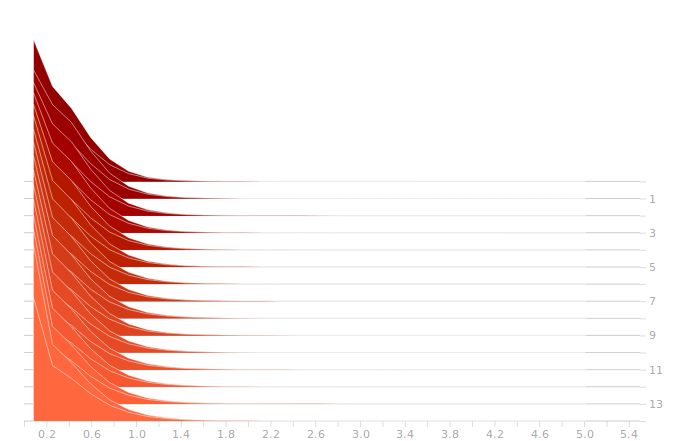
\includegraphics[width=0.5\linewidth]{part4/3CNN-merge3-128.png} \\ а}
	\end{minipage}
	\hfill
	\begin{minipage}[ht]{1\linewidth}
		\center{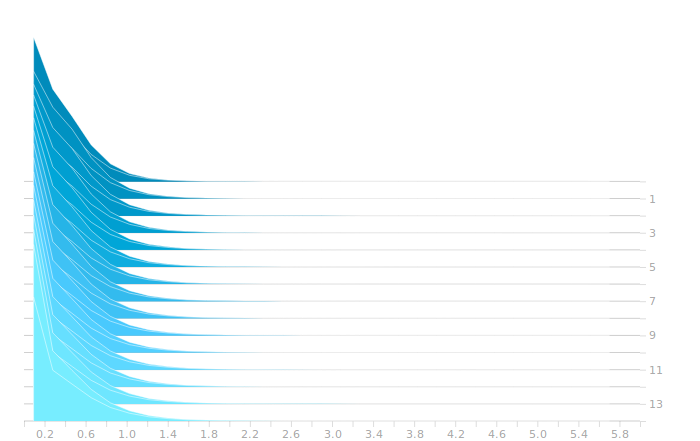
\includegraphics[width=0.5\linewidth]{part4/3CNN-merge3-256.png} \\ b}
	\end{minipage}
	\begin{minipage}[ht]{1\linewidth}
 		\center{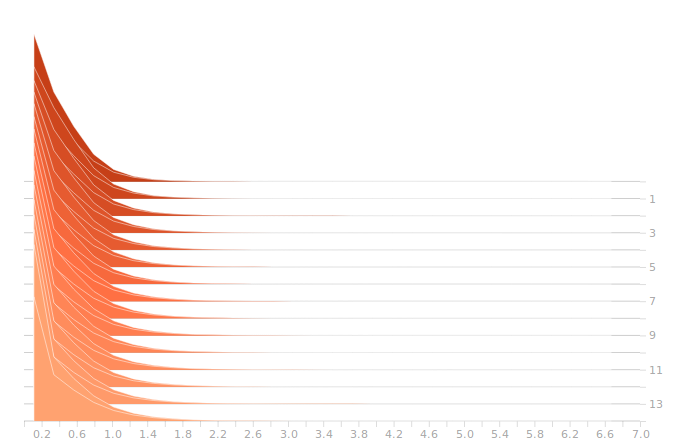
\includegraphics[width=0.5\linewidth]{part4/3CNN-merge3-512.png} \\ c}
	\end{minipage}
	\caption{Convolutional model (a) 128;(b) 256; (c) 512 filters for each sizes [3, 4, 5]. Histogram of merged layers}
	\label{img:category_crossentropy}  
\end{figure}


\begin{figure}[ht]
	\begin{minipage}[ht]{1\linewidth}
		\center{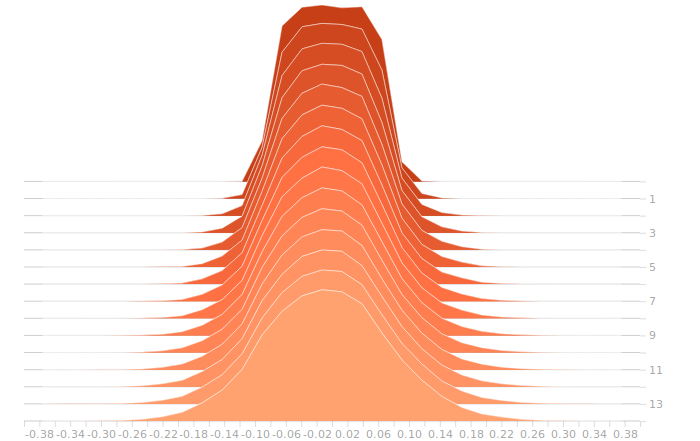
\includegraphics[width=0.5\linewidth]{part4/3CNN-dense-128.png} \\ а}
	\end{minipage}
	\hfill
	\begin{minipage}[ht]{1\linewidth}
		\center{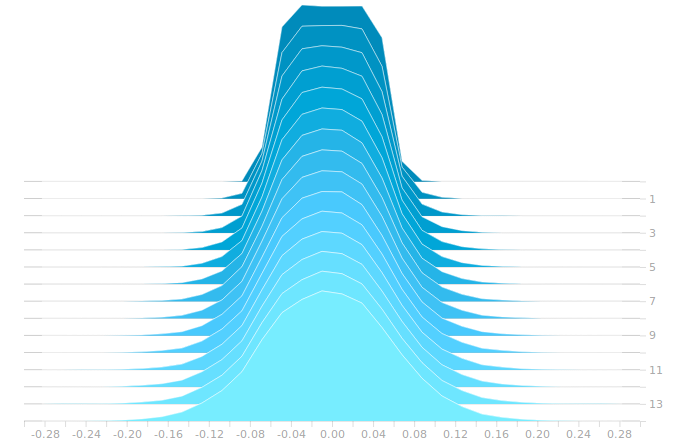
\includegraphics[width=0.5\linewidth]{part4/3CNN-dense-256.png} \\ b}
	\end{minipage}
	\begin{minipage}[ht]{1\linewidth}
		\center{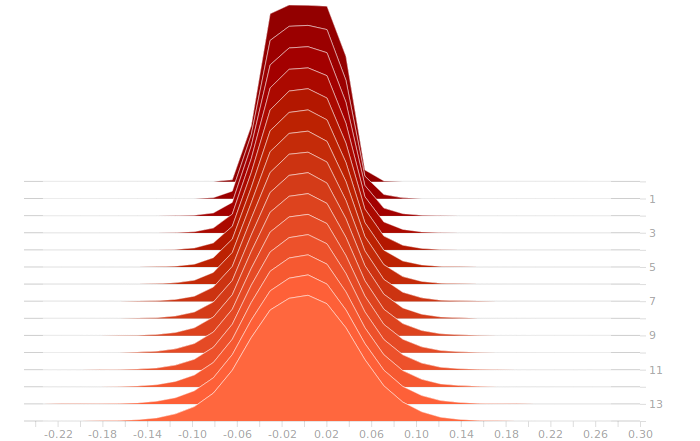
\includegraphics[width=0.5\linewidth]{part4/3CNN-dense-512.png} \\ c}
	\end{minipage}
	\caption{Convolutional model (a) 128;(b) 256; (c) 512 filters for each sizes [3, 4, 5]. Histogram of dense layers}
	\label{img:category_crossentropy}  
\end{figure}


\begin{figure}[ht] 
	\center
	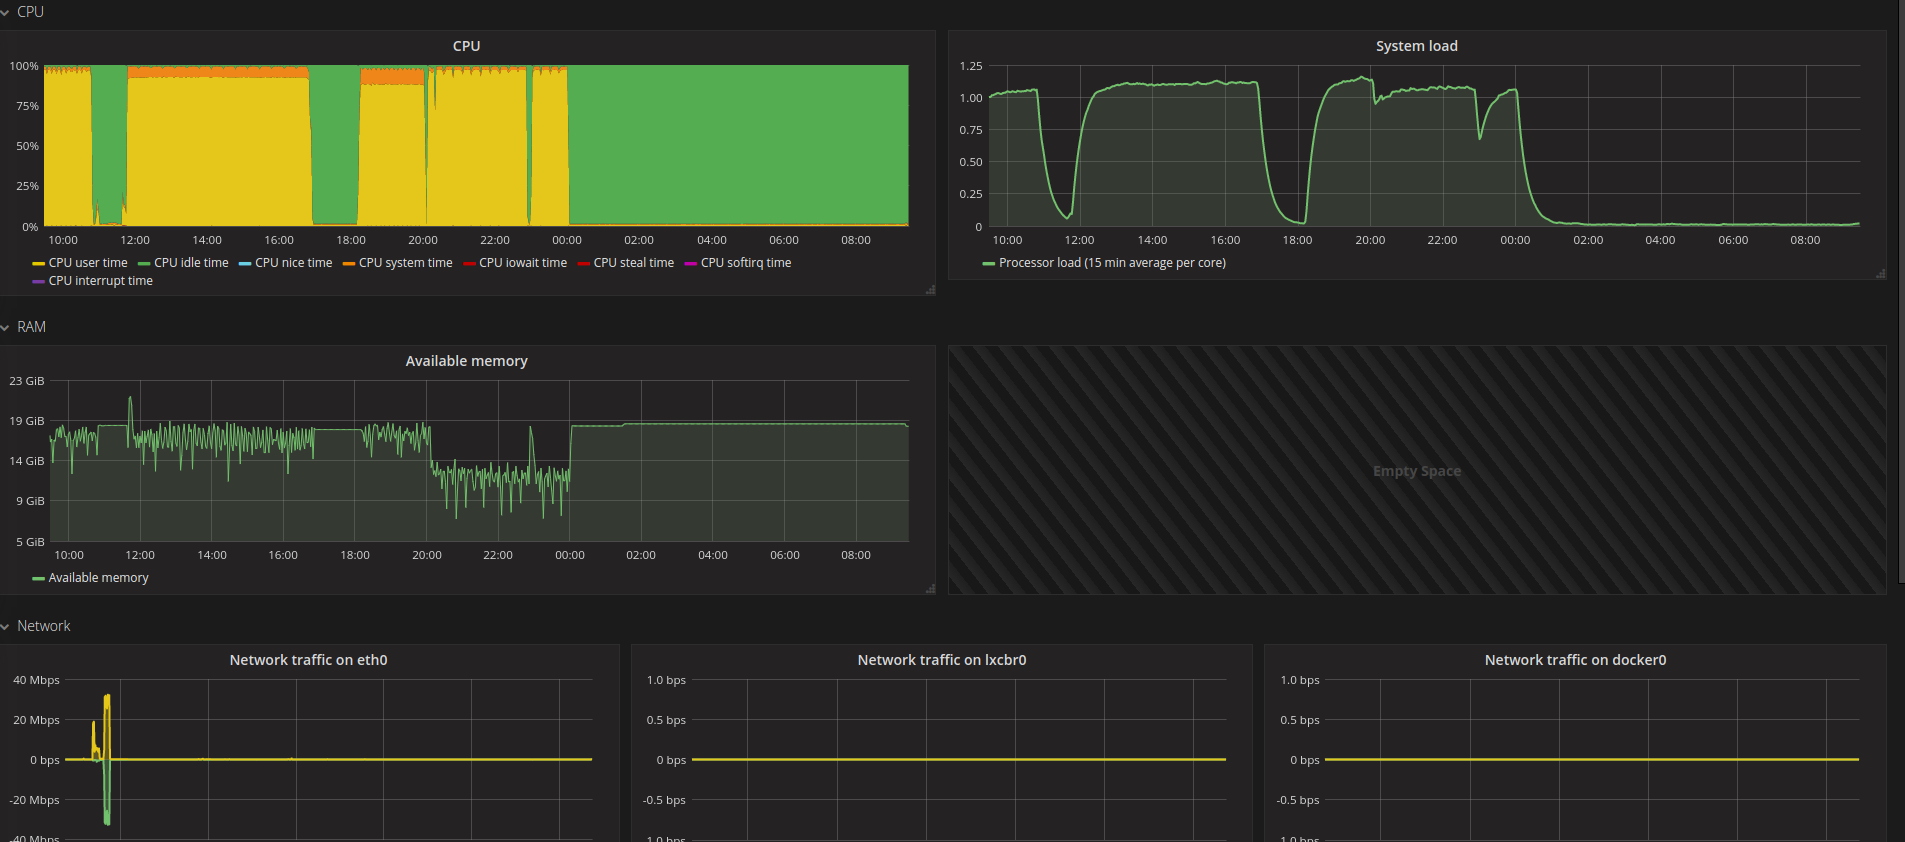
\includegraphics [scale=0.2] {part4/resources_CNN}
	\caption{CPU resources which were used while training CNN.} 
	\label{img:resources_CNN}  
\end{figure}






\section{Convolution neural network with different regularization} \label{sect4_3}

%'drop_1':  0.25,
%'drop_2': 0.25
%
%adam = Adam(lr=1e-4, 
%beta_1=0.9, 
%beta_2=0.999, 
%epsilon=1e-08, 
%decay=0.0)
%
%kernel_regularizer=regularizers.l2(0.001),
%
%blue-modified_epoch15_outdim183_nbfilters512_drop10.5_drop20.2
%grey-withl2regul_0.001_0.01_adam_epoch15_outdim183_nbfilters512_drop10.25_drop20.25
%pink-withl2regul_0.001_0.01_epoch15_outdim183_nbfilters512_drop10.25_drop20.25
%cyan-withl2regul_epoch15_outdim183_nbfilters512_drop10.25_drop20.25

\begin{figure}[ht]
	\begin{minipage}[ht]{1\linewidth}
		\center{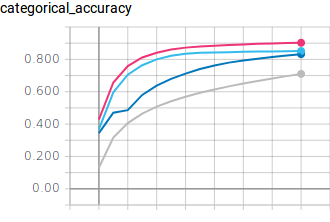
\includegraphics[width=0.5\linewidth]{part4/4CNN_train_category_accuracy}}
	\end{minipage}
	\hfill
	\begin{minipage}[ht]{1\linewidth}
		\center{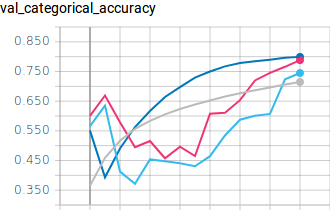
\includegraphics[width=0.5\linewidth]{part4/4CNN_val_category_accuracy}}
	\end{minipage}
	\caption{Models train and validation categorical accuracy by epochs}
	\label{img:3CNN_categorical_accuracy}  
\end{figure}


\begin{figure}[ht]
	\begin{minipage}[ht]{1\linewidth}
		\center{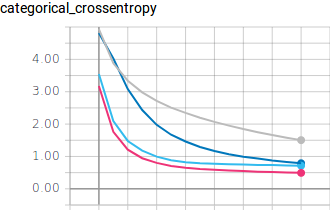
\includegraphics[width=0.5\linewidth]{part4/4CNN_train_category_crossentropy}}
	\end{minipage}
	\hfill
	\begin{minipage}[ht]{1\linewidth}
		\center{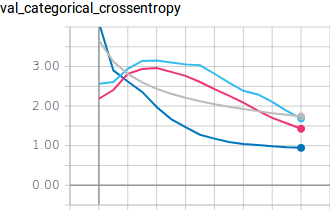
\includegraphics[width=0.5\linewidth]{part4/4CNN_val_category_crossentropy}}
	\end{minipage}
	\caption{Models train and validation category crossentropy by epochs}
	\label{img:3CNN_category_crossentropy}  
\end{figure}

\begin{figure}[ht]
	\begin{minipage}[ht]{1\linewidth}
		\center{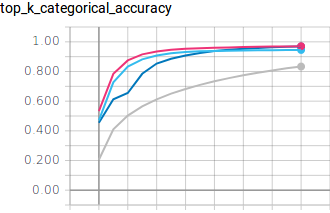
\includegraphics[width=0.5\linewidth]{part4/4CNN_train_top_k_accuracy}}
	\end{minipage}
	\hfill
	\begin{minipage}[ht]{1\linewidth}
		\center{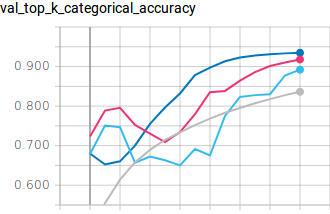
\includegraphics[width=0.5\linewidth]{part4/4CNN_val_top_k_accuracy}}
	\end{minipage}
	\caption{Models train and validation top k accuracy by epochs}
	\label{img:3CNN_top_k_accuracy}  
\end{figure}

\begin{figure}[ht] 
	\center
	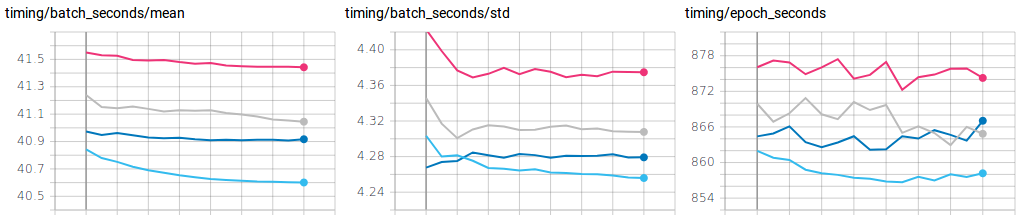
\includegraphics [scale=0.5] {part4/4CNN_timing}
	\caption{Models batch time by epochs} 
	\label{img:3CNN_timing}  
\end{figure}



\begin{figure}[ht]
	\begin{minipage}[ht]{1\linewidth}
		\center{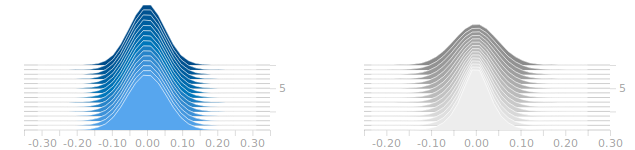
\includegraphics[width=0.5\linewidth]{part4/4CNN-conv-1.png} \\ а}
	\end{minipage}
	\hfill
	\begin{minipage}[ht]{1\linewidth}
		\center{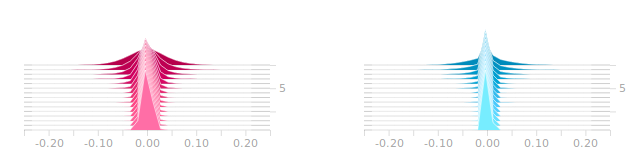
\includegraphics[width=0.5\linewidth]{part4/4CNN-conv-2.png} \\ b}
	\end{minipage}
	\caption{Convolutional model (a) 128;(b) 256; (c) 512 filters for each sizes [3, 4, 5]. Histogram of convolution layers}
	\label{img:category_crossentropy}  
\end{figure}


\begin{figure}[ht]
	\begin{minipage}[ht]{1\linewidth}
		\center{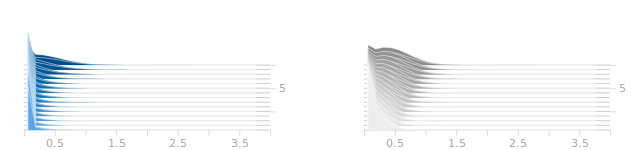
\includegraphics[width=0.5\linewidth]{part4/4CNN-merge3-1.png} \\ а}
	\end{minipage}
	\hfill
	\begin{minipage}[ht]{1\linewidth}
		\center{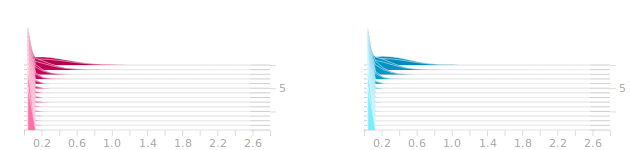
\includegraphics[width=0.5\linewidth]{part4/4CNN-merge3-2.png} \\ b}
	\end{minipage}
	\caption{Convolutional model (a) 128;(b) 256; (c) 512 filters for each sizes [3, 4, 5]. Histogram of convolution layers}
	\label{img:category_crossentropy}  
\end{figure}


\begin{figure}[ht]
	\begin{minipage}[ht]{1\linewidth}
		\center{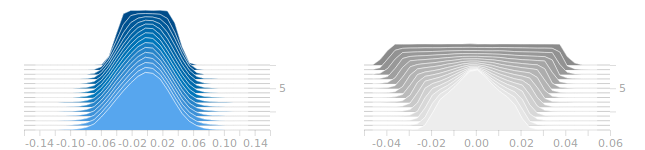
\includegraphics[width=0.5\linewidth]{part4/4CNN-dense-1.png} \\ а}
	\end{minipage}
	\hfill
	\begin{minipage}[ht]{1\linewidth}
		\center{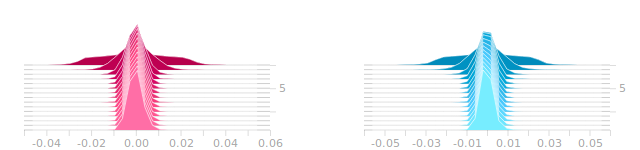
\includegraphics[width=0.5\linewidth]{part4/4CNN-dense-2.png} \\ b}
	\end{minipage}
	\caption{Convolutional model (a) 128;(b) 256; (c) 512 filters for each sizes [3, 4, 5]. Histogram of convolution layers}
	\label{img:category_crossentropy}  
\end{figure}

\section{Final model} \label{sect4_4}



\section{Classification results} \label{sect4_4}



